\chapter{Introduction}
\label{ch1:introduction}

    %\addcontentsline{toc}{chapter}{\protect\numberline{}Introduction}
    
     % Might be useful: http://www.emerson.emory.edu/services/latex/latex_162.html

\section{General context}

%Since its early days, humankind has always felt the desire to fly. 

%It was not until the World War I, when planes took a fundamental role in the last stages of the 

%In World War I, airplanes played a fundamental role 

% 15/10/2021, new goals to ELIMINATE CO2 by 2050: https://www.iata.org/en/pressroom/2021-releases/2021-10-04-03/

In the 20th century, the field of aeronautics has experienced a hectic growth since World War I (1914 - 1919), where airplanes played a fundamental role in aerial battles. The advances in military aviation led to the apparition of the first airlines and the birth of commercial aviation after the war. It was not, however, until World War II (1939 - 1945) when the greatest progresses were made: technological improvements resulted in larger, more efficient aircraft employed for surveillance, in air battles or for bombing purposes. After this period, airplanes used during the war were recycled with civil purposes to transport cargo and passengers. This supposed the beginning of a new era for commercial aviation which has continued to grow until nowadays, where air transportation is an essential activity in today's society.

The increasing relevance of commercial aviation has been possible due to advances in aeronautical technologies, from aircraft structures and flight control to propulsion systems. In the case of the latter, the birth of the jet engine in the 1930s supposed a milestone that marked the transition from propelled airplanes working with internal combustion engines to faster aircraft powered by gas turbines. Improvements in propulsion technologies have led to bigger, more efficient engines which can produce more power in order to drive bigger airplanes faster during longer times, hence covering longer distances. 

%However, despite today's propulsion technologies being more efficient than those from its origins, they are not extent of pollutant emissions. The increasing demand of commercial transportation in the last years, as well as the increasing general concern for the effects of greenhouse gases on climate change, has made the aeronautical engine manufactures to place emissions' reduction as a major constraint for engine design. In this respect, pollutant species such as CO, CO$_2$ and NO$_\mathrm{x}$, generated during the combustion process, are meant to be reduced. 

Despite today's propulsion technologies being more efficient than those from its origins, they are not exempt from producing emissions. Chemical species generated during the combustion process in gas turbines include CO$_2$, a greenhouse gas contributing to global warming, and CO and NO$_\mathrm{x}$, considered as pollutant emissions. In this respect, the increasing demand of commercial transportation and a rising general concern about the effects of climate change have placed the need of reducing emissions, as well as noise, as a major constraint for the development of aviation in the decades to come. The Advisory Council of Aeronautic Research in Europe (ACARE) has settled the goal to reduce the emissions per passenger/kilometre of CO$_2$ by 75 $\%$ and of NO$_\mathrm{x}$ by 90 $\%$ for the year 2050 with respect to the levels of 2000 \citepColor[acare_strategic_2017].

Emissions of NO$_\mathrm{x}$ are a big concern due to their harmful effect to health and environment (e.g. it is one of the main species producing acid rain). The evolution of aeronautical engines in the last decades have led to higher combustion temperatures and larger Overall Pressure Ratios (OPR), which help to reduce fuel consumption but increase the production of NO$_\mathrm{x}$. Engine manufacturers have worked on mitigating this increasing trend, as shown by the evolution of NO$_x$ emissions with OPR for several generations of engines in Figure \ref{fig:NOX_emissions_with_OPR}. It is shown how certified engines have succeeded in reducing emissions below the ICAO-CAEP regulatory limits. Nevertheless, the NO$_\mathrm{x}$ are still expected to grow due to the expanding aerial traffic demand. Figure \ref{fig:NOX_forecasts} displays the forecasts for several traffic scenarios, where it is shown the potential effect of technology advances in the emissions at 2040 (lower bounds) with respect to the case where current technologies (of year 2017) would be used (upper bounds). Therefore, in order to maintain the emissions below a certain level and hence accomplish ACARE's goals, substantial efforts are being done. One way of achieving this is by controlling and improving the combustion process, since NO$_\mathrm{x}$ are produced at high temperatures. For this purpose, the aeronautical community is working towards new combustion chambers and injection processes aiming at creating \textbf{lean combustion}.

\begin{figure}[h!]
	\centering
	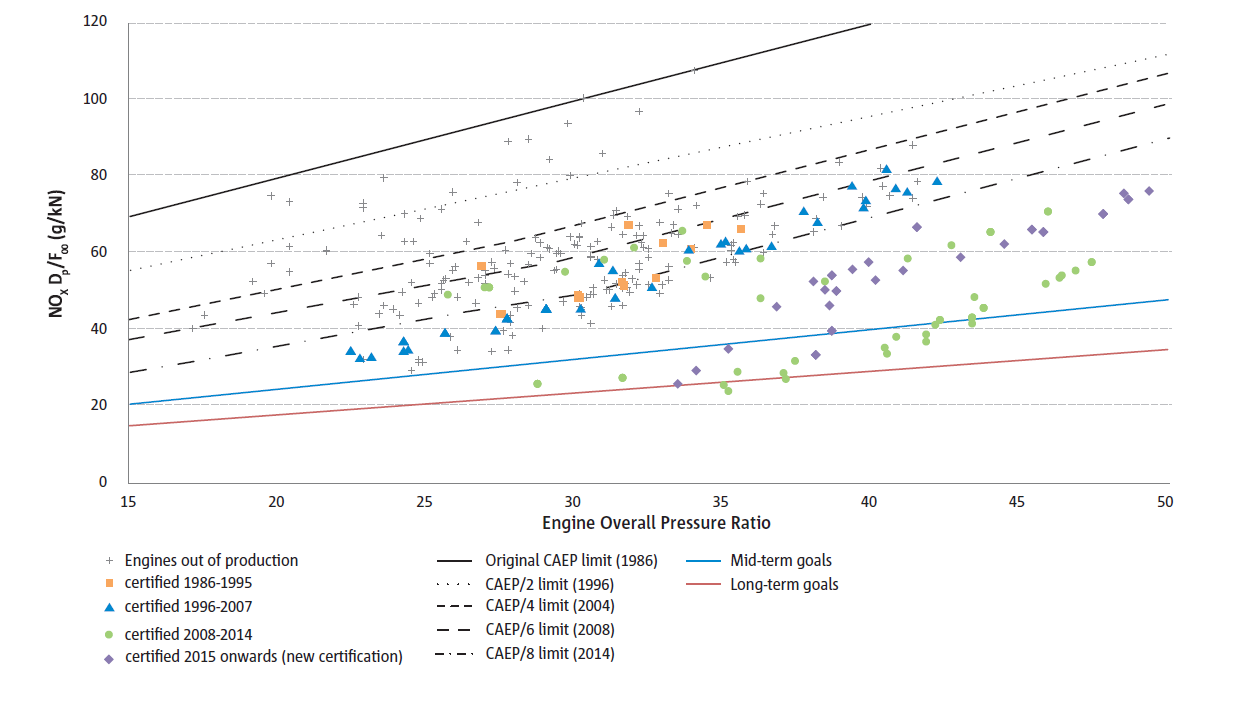
\includegraphics[scale=0.6]{./part0_intro/NOx_emissions_with_OPR}
	\caption[Evolution of NO$_x$ emissions with several generations of aircraft engines]{Evolution of NO$_x$ emissions with several generations of aircraft engines. Source: \citepColor[easa_european_2019]}
	\label{fig:NOX_emissions_with_OPR}
\end{figure}

\begin{figure}[h!]
	\centering
	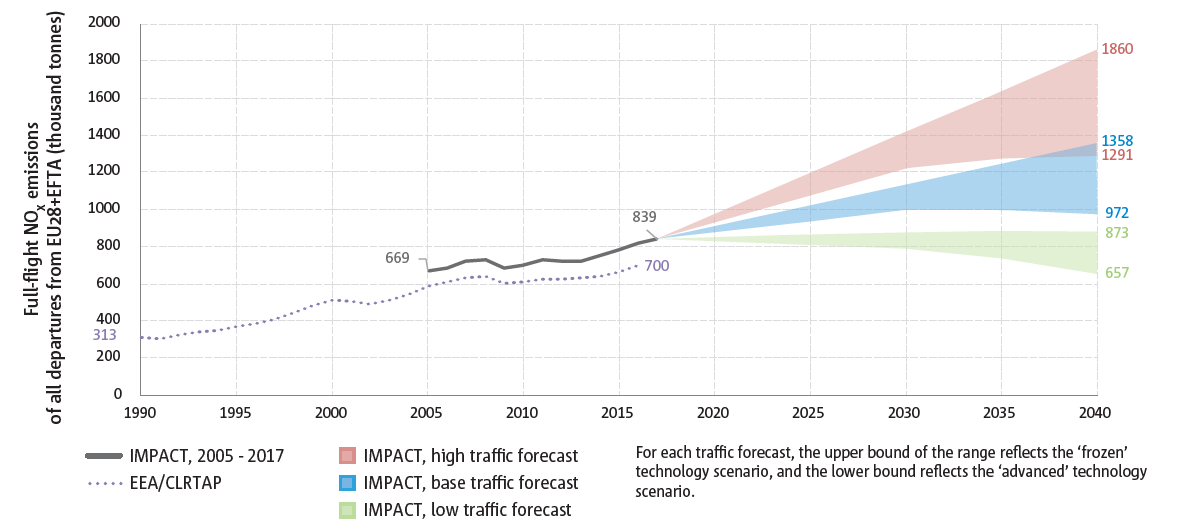
\includegraphics[scale=0.6]{./part0_intro/NOx_emissions_forecast_report2019}
	\caption[NO$_x$ emission forecasts from 2017 to 2040]{NO$_x$ emission forecasts from 2017 to 2040. Source: \citepColor[easa_european_2019]}
	\label{fig:NOX_forecasts}
\end{figure}


\section{Lean combustion in aeronautical gas turbines}

%Conventional combustors used to introduce only a small portion of air ($\sim 30 \%$ ) with the liquid injection system, and the rest was introduced through secondary holes located downstream (see Figure \ref{fig:combustor_conventional}). As a consequence, com

%\begin{figure}[h!]
%	\centering
%	\includegraphics[scale=0.6]{./part0_intro/combustor_conventional}
%	\caption{Conventional combustor. Source: \citeColor[lefebvre_gas_2010].}
%	\label{fig:combustor_conventional}
%\end{figure}

%With the objective of reducing NO$_\mathrm{x}$ emissions in aeronautical engines, the community has worked towards the implementation of concepts aiming at producing lean combustion. 

The motivation for developing lean systems is shown in Figure \ref{fig:NOX_motivation_and_RQL} left. At lean regimes (i.e. with an excess of air), the flame temperature is lower and, consequently, NO$_\mathrm{x}$ formation is reduced. At the same time, emissions of CO, hydrocarbons (HC) and soot are also diminished at this regime (provided that the air excess is not too high, or the emissions will start to grow again). On the other hand, operating at lean regimes will make the system more prone to thermoacoustic instabilities and will place it closer to the the limit of lean blow-out (LBO), hindering ignition and relight capabilities. 

One of the first developed concepts aiming at reducing emissions was the \textbf{Rich-Burn, Quick-Quench, Lean-Burn} (\textbf{RQL})  \citepColor[novick_low_1981]. RQL systems split the combustion process in three stages. Firstly combustion begins in a fuel-rich primary zone close to the injector, where the NO$_\mathrm{x}$ rate is low (see Figure \ref{fig:NOX_motivation_and_RQL} left). Then, a quick mixing of the unburnt fuel takes place with fresh air to finally burn in lean conditions. This procedure allows to decrease NO$_\mathrm{x}$ emissions as depicted by the low-NO$_\mathrm{x}$ route in Figure \ref{fig:NOX_motivation_and_RQL} right. However, a fine and complete fuel atomization is needed so that a fast mixing takes place; otherwise, unburnt fuel could produce extra smoke and soot in the rich-burn region \citepColor[el-asrag_simulation_2007]. This hinders the proper operation of RQL chambers in regimes where fuel can hardly be atomized, such as during altitude relight.

\newpage

\begin{figure}[h!]
	\centering
	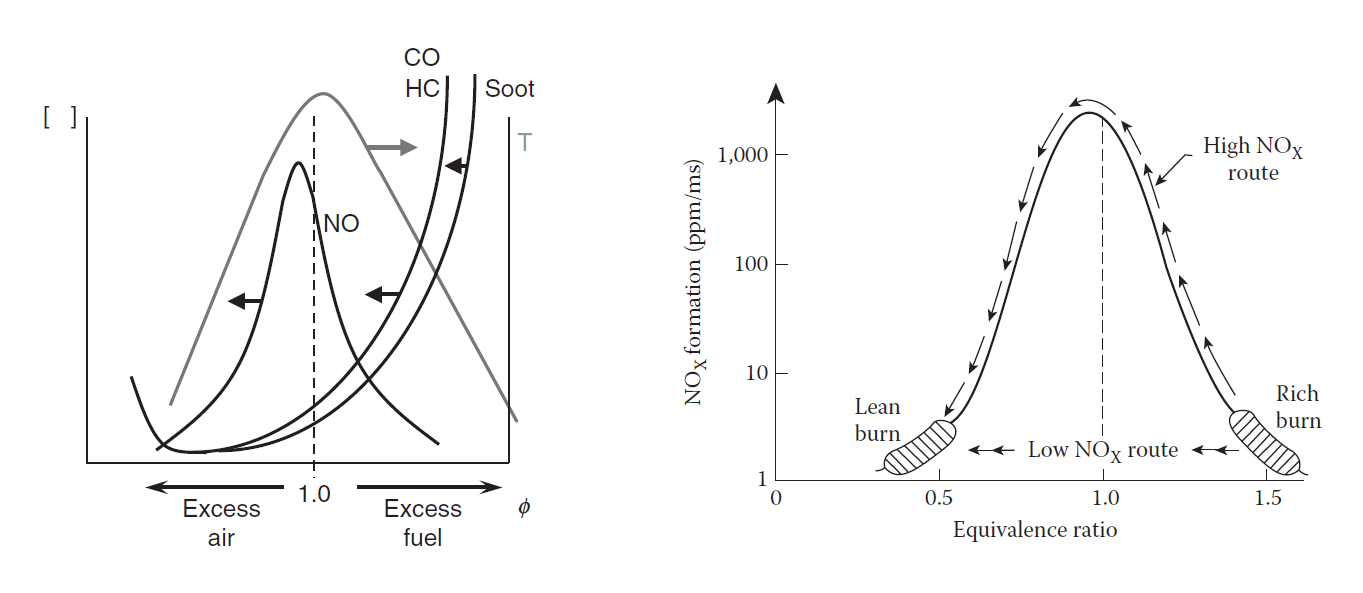
\includegraphics[scale=0.65]{./part0_intro/NOX_motivation_and_RQL}
	\caption[Motivation for low-NOx combustion]{Motivation for low-NOx combustion. \textsl{Left}: Temperature and species concentration variation with stoichiometric ratio in combustion chambers. Source: \citeColor[dunn-rankin_lean_2008]. \textsl{Right}: NOx formation in Rich-Burn, Quick-Quench, Lean-Burn (RQL) concepts. Source: \citeColor[lefebvre_gas_2010].}
	\label{fig:NOX_motivation_and_RQL}
\end{figure}

The need of reducing NO$_\mathrm{x}$ emissions to the levels settled by authorities led to the development of lean combustion strategies, usually referred as low-NO$_\mathrm{x}$ \citepColor[tacina_low_1990]. In order to foster lean combustion, low-NO$_\mathrm{x}$ concepts introduce an excess of air at the vicinity of the injector: around $70 ~\%$ of air is introduced in the combustion chamber at this location (primary zone), while the rest is injected further downstream for effusion cooling. Compared to conventional combustors, where around $30 ~\%$ of air is injected in the primary zone and the rest is introduced downstream through dilution holes, this allows to reduce the length of the combustion chamber and hence the residence time of combustion, directly linked to NO$_\mathrm{x}$ formation \citepColor[lefebvre_gas_2010]. Furthermore, operating directly at lean regimes will also reduce the formation of soot and CO emissions, which is the main disadvantage of RQL. One of the first lean combustion concepts is the \textbf{Lean Direct Injection} (\textbf{LDI}) technology \citepColor[tacina_low_1990], where fuel is directly introduced into the reaction zone without previous premixing. Lower peak temperatures and residence times are obtained, hence reducing pollutant formation. Contrarily, LDI concepts can produce a non-uniform combustion if mixing is not complete. In this respect, the \textbf{Lean Premixed Prevaporized} (\textbf{LPP}) technology appeared to palliate this issue \citepColor[bittlinger_high_1999]: a premixing length is added before the reaction zone, so that complete evaporation of fuel and mixing can take place before triggering combustion. LPP concepts need, however, a longer combustion chamber to account for the dilution zone, and are more prone to suffer autoignition, flashback and thermoacoustic instabilities.

A good trade-off between both LDI and LPP is obtained with \textbf{Multi-Staged Fuel Injection} (MSFI) \citepColor[pehanhoat_low_2006]. Fuel is introduced in the combustion chamber through two main stages: a \textbf{pilot stage} for flame stabilization purposes, and a \textbf{take-off stage} (also called multipoint) where the most of premixing takes place (see Figure \ref{fig:foust_TAPS} left). The combination of both injection systems creates a flame that burns in lean conditions and reduces combustion instabilities compared to other low-NO$_\mathrm{x}$ concepts \citepColor[barbosa_time_2009]. The percentage of fuel introduced through each stage can be controlled in order to optimize the combustion performance depending on the flight phase: this procedure is called staging. Considerable reductions in emissions can be obtained with MSFI in conditions where most of NO$_\mathrm{x}$ is produced, such as climb and cruise. Figure \ref{fig:foust_TAPS} right shows the improvements in pollution of a multi-staged fuel injector named Twin Annular Premixing Swirler (TAPS) \citepColor[foust_development_2012] compared to a RQL combustor.

\begin{figure}[h!]
	\centering
	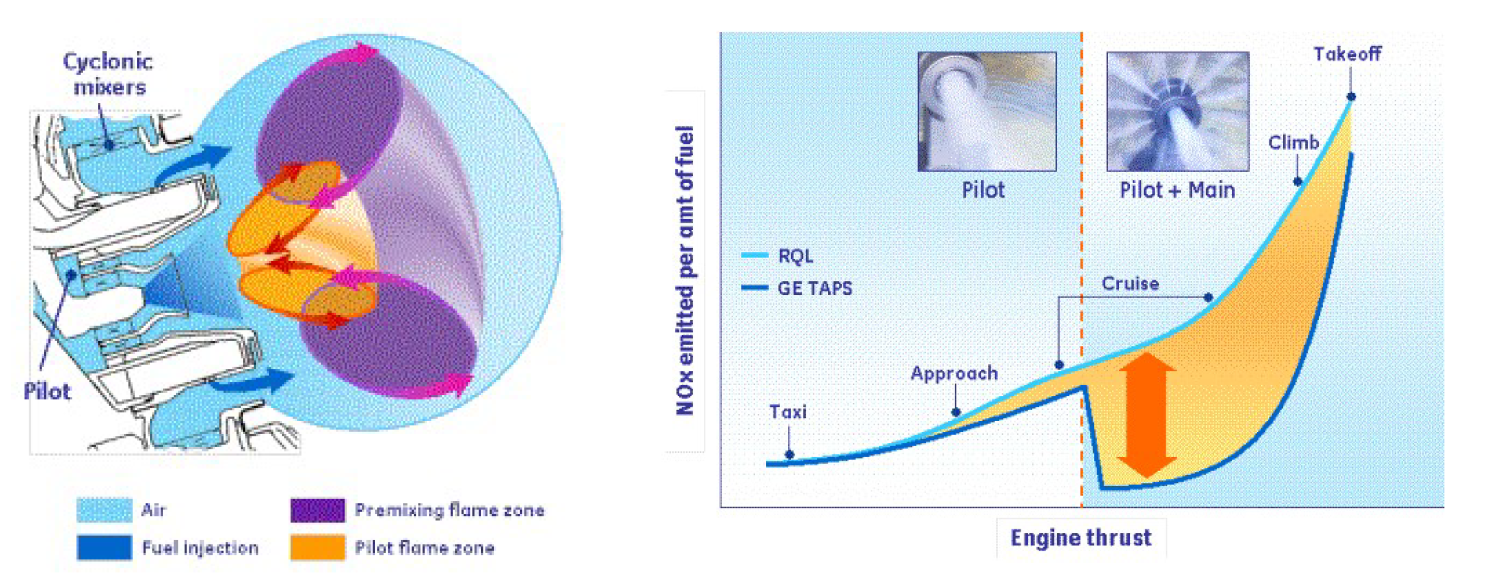
\includegraphics[scale=0.52]{./part0_intro/foust_TAPS}
	\caption[The TAPS concept]{The TAPS concept. \textsl{Left}: regions in a multi-staged injection system from a TAPS concept. \textsl{Right}: effect of multi-staged injection in NO$_\mathrm{x}$ emissions from a TAPS concept compared to a RQL system. Source: \citeColor[foust_development_2012].}
	\label{fig:foust_TAPS}
\end{figure}

MSFI are a promising technology for fuel injection in aeronautical combustors, and manufacturers such as Safran are working in developing these systems for their application in future engines. Since their main characteristic is fuel staging, processes prior to combustion (e.g. injection, atomization and mixing) are fundamental for MSFI performance, and their proper comprehension is paramount to optimize such systems. The next sections makes a review on the two-phase flow physical mechanisms of injection and atomization relevant to these injection systems.


\section{Fuel injection technology}
\label{sec:ch1_fuel_injection_technology}

Figure \ref{fig:multipoint_injector_snecma} shows a MSFI injector and the atomization mechanisms present in these systems. Fuel is injected through two inlets: a central nozzle (the pilot stage), where fuel is injected with a pressure-swirl atomizer spreading as a \textbf{hollow cone} spray, and the multipoint injectors located in a crown around the central injector (the take-off stage), where fuel is injected in a \textbf{jet in crossflow} configuration (JICF). As seen in the figure, these two injection systems will produce liquid atomization shortly after the injection location. Furthermore, a third breakup mechanisms is present if the opening angle of the hollow cone is large enough: in such cases, liquid can impinge the walls of the injector and break due to the interaction between the liquid, aerodynamics and wall, forming an \textbf{airblast} spray. As a consequence of these three atomization mechanisms, a dispersed spray will be formed further downstream the injection chamber. This dispersed spray will be later able to evaporate, mix with the surrounding air and burn in the combustion process.

%\begin{figure}[ht]
%     \centering
%     \begin{subfigure}[b]{0.45\textwidth}
%         \centering
%         \includeinkscape[inkscapelatex=false,scale=0.35]{./part0_intro/multipoint_injector_snecma}
%     \end{subfigure}
%     %\hfill
%     \begin{subfigure}[b]{0.45\textwidth}
%         \centering
%          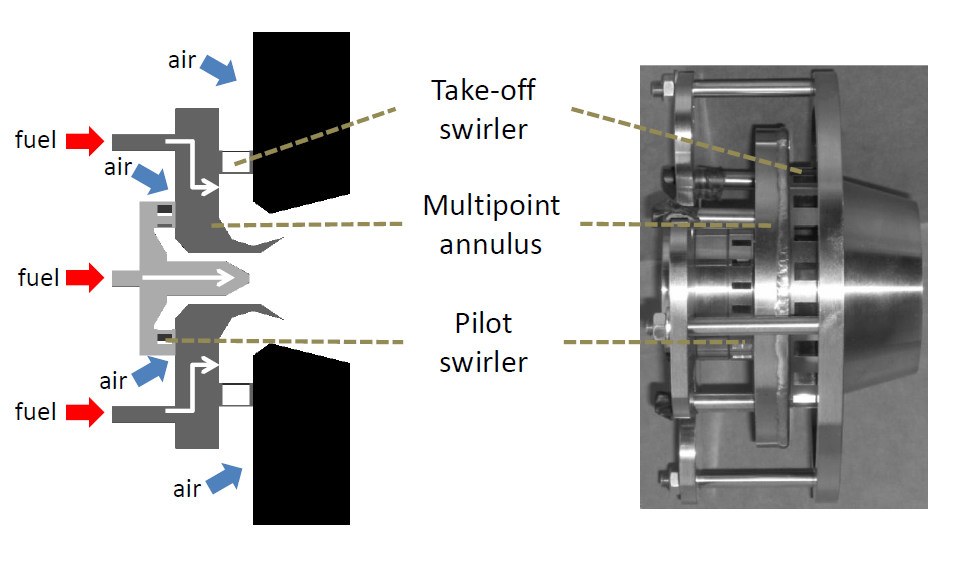
\includegraphics[scale=0.5]{./part0_intro/BIMER_swirler}
%     \end{subfigure}
%        \caption{\textsl{Left}: Size histogram evolution with accumulation time of droplets. \textsl{Right}: comparison of two droplet size histograms from two consecutive time instants.}
%	% See: https://stackoverflow.com/questions/35210337/can-i-plot-several-histograms-in-3d/35225919
%        \label{fig:multipoint_injectors}
%\end{figure}



\begin{figure}[ht]
     \centering
     \includeinkscape[inkscapelatex=false,scale=0.55]{./part0_intro/multipoint_injector_snecma}
      \caption[Multipoint injector from SNECMA showing the atomization mechanisms present in MSFI systems]{Multipoint injector from SNECMA showing the atomization mechanisms present in MSFI systems. Source: \citeColor[jaegle_large_2009]}
      \label{fig:multipoint_injector_snecma}
\end{figure}

A view of the several multiphysical phenomena found within a combustor is shown in Figure \ref{fig:JICF_multiphysics} with an example of reactive liquid JICF. Liquid fuel is injected through the injection nozzle as a coherent jet. Instabilities start taking place after injection which will eventually break the jet into large blobs and ligaments during a process known as \textbf{primary atomization} (or primary breakup). Resulting liquid structures will then break into smaller droplets during \textbf{secondary atomization} (or secondary breakup) until the droplets are in equilibrium with the surrounding air and reach a small size and a spherical shape. As a consequence of the atomization process, the specific surface of the spray (i.e. the amount of liquid surface which is in contact with the continuous gas) is large and then \textbf{evaporation} can take place. Gaseous fuel can then \textbf{mix} with the surrounding air  to produce an ignitable mixture that can finally burn in a \textbf{combustion} process. Other physical mechanisms are found taking place simultaneously, such as drop-drop interactions, wall-drop interactions and droplet combustion. All these processes are generally found within gas turbines.

\begin{figure}[ht]
     \centering
     \includeinkscape[scale=0.75]{./part0_intro/JICF_multiphysics}
      \caption{Multi-physics phenomena in a reactive jet in crossflow. }
      \label{fig:JICF_multiphysics}
\end{figure}

As illustrated in Figures \ref{fig:multipoint_injector_snecma} and \ref{fig:JICF_multiphysics}, the atomization process is responsible for the generation of droplets. It is necessary that the size of these droplets is small enough so that the liquid specific surface is large and fuel can burn efficiently. Otherwise, unburnt fuel and inefficient combustion can increase the production of pollutants such as NO$_x$ and soot. Understanding the driving mechanisms of atomization is therefore essential for the correct design of atomizers and injectors. However, its study is not trivial due to its multi-scale nature, since atomization involves a wide range of length-scales from the injector size to the diameter of the smallest droplets, with a difference of several orders of magnitude.  The rest of this section is then devoted to introducing the fundamentals of atomization and the jet in crossflow phenomenon, which is of special interest for MSFI systems and constitutes the main core of this thesis.

\subsection*{The atomization process}

After liquid injection, atomization is the mechanism through which coherent, dense liquid is fractured into smaller liquid structures. \citeColor[lefebvre_atomization_2017] define atomization as "\textsl{the process by which a liquid jet or sheet is disintegrated by the kinetic energy of the liquid, by the exposure to
high-velocity air or gas, or by mechanical energy applied externally through a rotating or vibrating device} (sic)". Its purpose is to increase the liquid specific surface to allow for fuel evaporation.

Atomization is initially triggered by instabilities which are found naturally in liquids jets. \citeColor[rayleigh_instability_1878] found that jet breakup into smaller drops is produced due to the growth of small disturbances in the liquid. Instabilities are amplified by the aerodynamic interaction with the surrounding air, enhancing the energy transfer between both phases. Turbulence in the jet also amplifies these disturbances: if liquid is injected in a high turbulent state, atomization will occur promptly and breakup will be governed by the aerodynamic forces, while if the jet is injected at low speed the breakup will be governed by surface tension and capillary forces, and the breakup morphology will be different. Regimes of atomization are distinguished according to two main dimensionless numbers, the \textbf{Reynolds number} $Re$ and the \textbf{Weber number} $We$:

\begin{equation}
\label{eq:ch1_intro_Re_and_We_general_definitions}
	Re = \frac{\rho u D}{\mu} ~~~~~~ ;  ~~~~~~ We = \frac{\rho u^2 D}{\sigma}
\end{equation}

where $\rho$ is density, $\mu$ the viscosity, $\sigma$ the surface tension, $u$ is a characteristic velocity (usually the liquid velocity or the relative velocities between liquid and gas), $D$ a characteristic length (usually the nozzle diameter or the droplet size). The Reynolds number represents the ratio between the aerodynamic forces and the viscous ones: a high $Re$ indicates a high turbulent state and a dominance of inertia as the main breakup mechanism, while a low $Re$ means laminar flow and a predominant role of viscosity. The Weber number defines the relative importance of aerodynamic forces with respect to capillary forces. From these definitions applied to the liquid phase, $Re_l$ and $We_l$, a third ratio measuring the relative importance between viscous and surface tension forces, called \textbf{Ohnesorge number}, can be defined:

\begin{equation}
Oh = \frac{\sqrt{We_l}}{Re_l} = \frac{\mu_l}{\sqrt{\rho_l D \sigma}}
\end{equation}

\begin{figure}[h!]
	\centering
	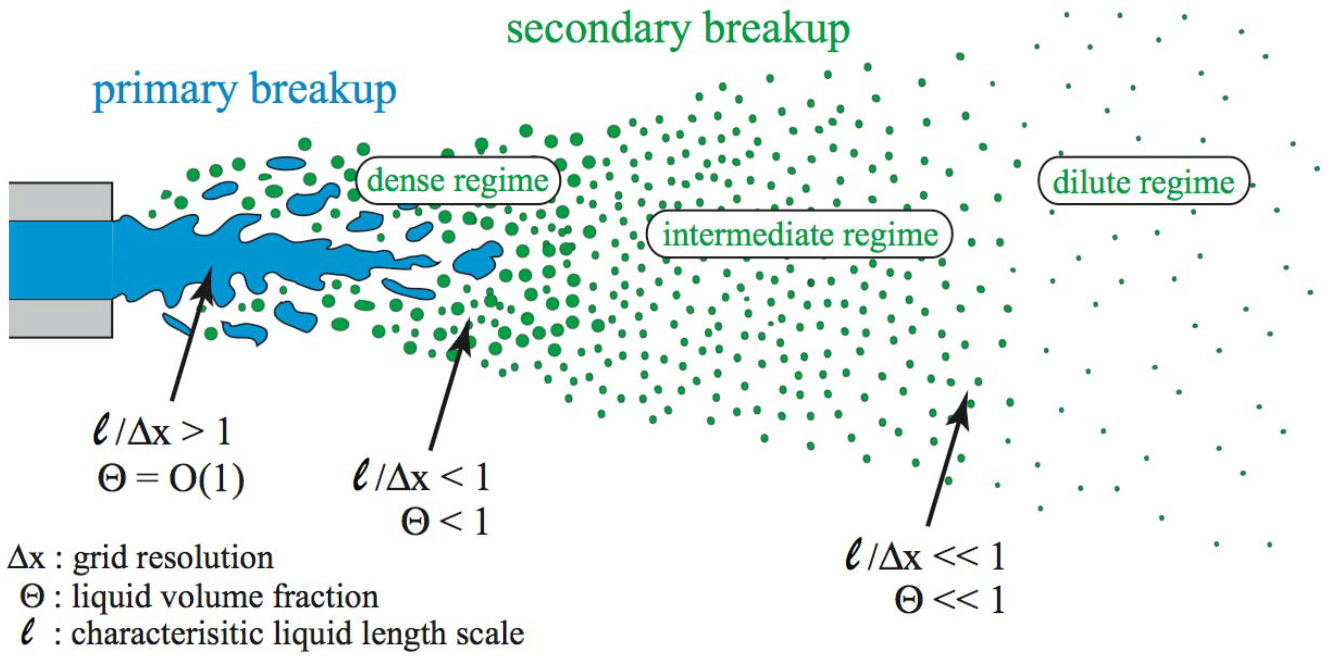
\includegraphics[scale=0.5]{./part0_intro/atomization-regimes-scheme}
	\caption[Atomization breakup regimes]{Atomization breakup regimes. Source: \citeColor[herrmann_modeling_2003]}
	\label{fig:atomization_regimes_herrmann}
\end{figure}

Figure \ref{fig:atomization_regimes_herrmann} illustrates liquid jet injection and atomization. The latter is generally divided by the scientific community in two different regimes, which are commonly found in all disintegrations of jets independently of the injection methodology:

\begin{itemize}

	\item \textbf{Primary atomization} is the process by which a liquid jet or sheet breaks from a dense structure into primary structures such as large blobs and ligaments. It is highly dependent on the injector system (pressure-swirl atomizer, jet in crossflow, airblast, etc.) and its characteristics (internal geometry, discharge pressure, discharge coefficient, liquid turbulent state, etc.). As shown in Figure \ref{fig:atomization_regimes_herrmann}, regions where primary atomization takes place are characterized by high characteristic length scales $l$ (larger than the grid resolution) and high liquid volume fractions, characteristics of the \textbf{dense regime}. Numerical methods targeted to solve for primary atomization are addressed in Chapter \ref{ch2:numerical_methods_resolved_atomization}. 
	
	Several regimes of primary atomization are distinguished, classified according to the liquid flow state. These regimes, shown in Figure \ref{fig:regimes_atomization_primary}, depend on $Re_l$ and $Oh$ based on the liquid velocity and on the injection diameter $d_0$. As shown, for a fixed value of $Oh$ the governing breakup mechanisms changes if the injection velocity increases (i.e. if $Re_l$ is increases, so turbulence will play a more important role). For the $\textbf{Rayleigh regime}$ at low values of $Re_l$, surface tension is the responsible for creating axisymmetric oscillations of the jet with large wavelengths that will make it break into structures larger than the nozzle diameter. Aerodynamic effects are negligible, being capillary forces the leading physical phenomena, and breakup occurs at several nozzle diameter locations downstream the injection point. As $Re_l$ increases, the relative velocity between the liquid and gas phases is higher and aerodynamic forces cannot be neglected. These ones contribute to the destabilizing waves that create droplets of the size of the nozzle diameter and lead a faster atomization, yet still occurring at several diameters downstream the injector (\textbf{first wind induced regime}). An slightly larger $Re_l$ will swift the dominant breakup role of capillary forces to inertial ones, the wavelenghts of instabilities being amplified by liquid turbulent eddies which break the jet into droplets smaller than the injection nozzle (\textbf{second wind induced}). Finally, at even larger values of $Re_l$ capillary forces can be neglected and the breakup is solely governed by aerodynamics, creating small droplets generated right at the nozzle exit (\textbf{atomization regime}).

	\begin{figure}[h!]
		\centering
		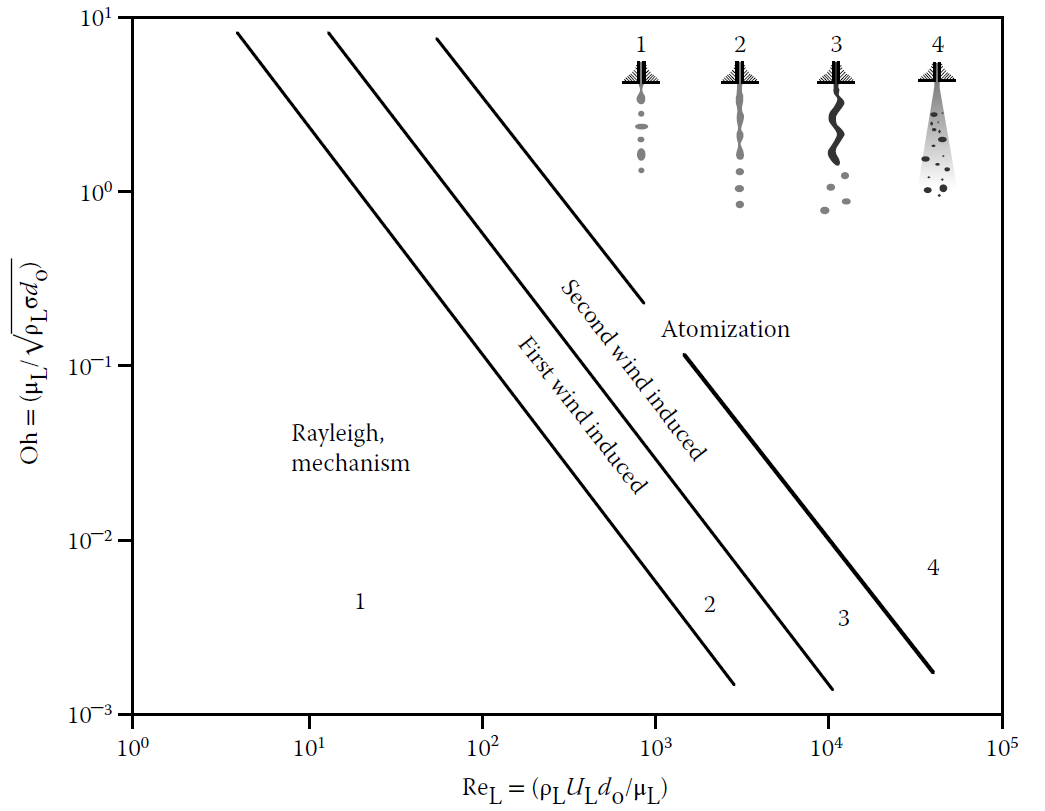
\includegraphics[scale=0.45]{./part0_intro/regimes_atomization_primary}
		\caption[Primary atomization regimes in jets]{Primary atomization regimes in jets. Source: \citeColor[lefebvre_atomization_2017]}
		\label{fig:regimes_atomization_primary}
	\end{figure}

	
	\item \textbf{Secondary atomization} occurs after primary atomization, once the main liquid structures have been ejected from the jet and are broken into smaller ones. Injector characteristics and the turbulent state of the coherent liquid do not play a fundamental role anymore: it is the interaction between the liquid structures and the surrounding air what dominates secondary breakup. Figure \ref{fig:atomization_regimes_herrmann} sketches how secondary atomization disintegrates the liquid structures until a developed spray composed of spherical droplets that do not further break. During secondary atomization, the spray undergoes a transition from the dense regime found in primary atomization to a \textbf{dilute regime} where the characteristic length scales of liquid (i.e. the droplets diameters) are very small compared to the injector diameter. In this regime, the liquid volume fraction is very low. Between the dense and dilute regimes, an \textbf{intermediate regime} can be defined where values of volume fraction and comprised between those of the dense and dilute ones. The lower liquid volume fractions and small sizes (usually smaller than the mesh resolution) found in these regimes require numerical resolution through methods different from those devoted to simulate primary atomization. Such methods are introduced in Chapter \ref{ch3:disperse_phase_methods}.
	
	As the main phenomenon governing secondary atomization is the interaction between the liquid and the gas, this process can be characterized by means of the Weber number based on the relative velocity between phases:
	
	\begin{equation}
	We = \frac{\rho_g u_\mathrm{rel}^2 r}{\sigma} 
	\end{equation}
	
	where $u_\mathrm{rel} = | \textbf{u}_l - \textbf{u}_g  |$ and $r$ is a characteristic length of the liquid structures (the radius for spherical droplets). Different regimes of secondary atomization, universal for any injector geometry and injection system, are depicted in Figure \ref{fig:regimes_atomization_secondary}. For large numbers of $We$ (i.e. high relative velocities and/or large length scales) the breakup is \textbf{catastrophic}, and particles are disintegrated into a large number of very small droplets due to shear forces causing stripping. As $We$ decreases the topology of structures found during atomization changes and breakup becomes less aggressive. For small values of $We$, particles split into a small number of droplets due to \textbf{bag} or \textbf{vibrational} breakups. For $We < 12$, breakup hardly occurs and droplets are said to be in equilibrium with the surrounding air: atomization is complete. This value is called the \textbf{critical Weber number}. 
	
	The interactions among droplets (drop-drop) and between droplets and walls (drop-wall), both illustrated in Figure \ref{fig:JICF_multiphysics} also produce secondary atomization with different governing mechanisms than the drop-air interaction. These particular phenomena are not addressed in this thesis and hence they will not be further discussed.
	
	\begin{figure}[h!]
		\centering
		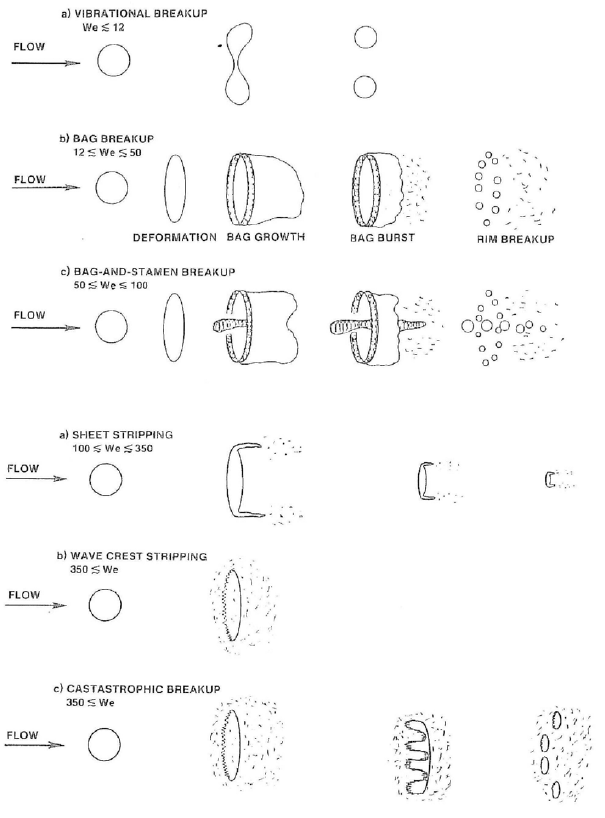
\includegraphics[scale=1.0]{./part0_intro/regimes_atomization_secondary}
		\caption[Secondary atomization regimes]{Secondary atomization regimes. Source: \citeColor[pilch_use_1987]}
		\label{fig:regimes_atomization_secondary}
	\end{figure}

\end{itemize}



\subsection*{Liquid jet in crossflow}

Contrarily to secondary atomization, whose behaviour is not influenced by the injection system, primary atomization is highly dependent on the injector configuration. As a consequence, different liquid structures and characteristic sizes are present in MSFI systems due to the different atomization mechanisms (see Figure \ref{fig:multipoint_injector_snecma}). One characteristic breakup mechanism of MSFI is the one from the take-off stage, which injects fuel in a particular configuration known as liquid jet in crossflow (JICF). This section discusses primary atomization and the influencing parameters of JICF, which is the injection configuration studied in this thesis.

In a liquid JICF, a stream of air flows perpendicularly to the direction of liquid injection, as shown in Figure \ref{fig:JICF_multiphysics}. The liquid jet leaves the nozzle and bends towards the crossflow direction, undergoing primary and secondary atomization. Consequently, a developed spray is formed further downstream the injection nozzle. The aerodynamic interaction with the surrounding air is of paramount importance: it influences the jet breakup, vertical penetration and the atomization process, which will eventually affect the mixing process prior to combustion in reactive applications.

%\subsubsection*{Breakup process}

The atomization process in liquid JICF has been investigated experimentally by several authors \citemColor[adelberg_breakup_1968,wu_breakup_1997,becker_breakup_2002,ragucci_trajectory_2007,freitag_spray_2008]. These studies have generally identified two main mechanisms of primary breakup:

\begin{itemize}

	\item \textbf{Column breakup}. Surface waves on the liquid column start to grow until the jet breaks into ligaments, which eventually turn into droplets during secondary atomization. An example is shown in Figure \ref{fig:JICF_breakup_mechanisms_freitag} left, showing the surface waves caused by instabilities. This type of breakup occurs when the aerodynamic interaction is not too strong (low relative liquid-air velocities).

\item \textbf{Surface breakup}. A strong aerodynamic interaction (large relative liquid-air velocity) produces the disintegration of the liquid jet through shear forces. Small droplets are directly
stripped off the sides of the liquid column. Surface breakup can be appreciated in Figure \ref{fig:JICF_breakup_mechanisms_freitag} right. 

\end{itemize}

\begin{figure}[h!]
	\centering
	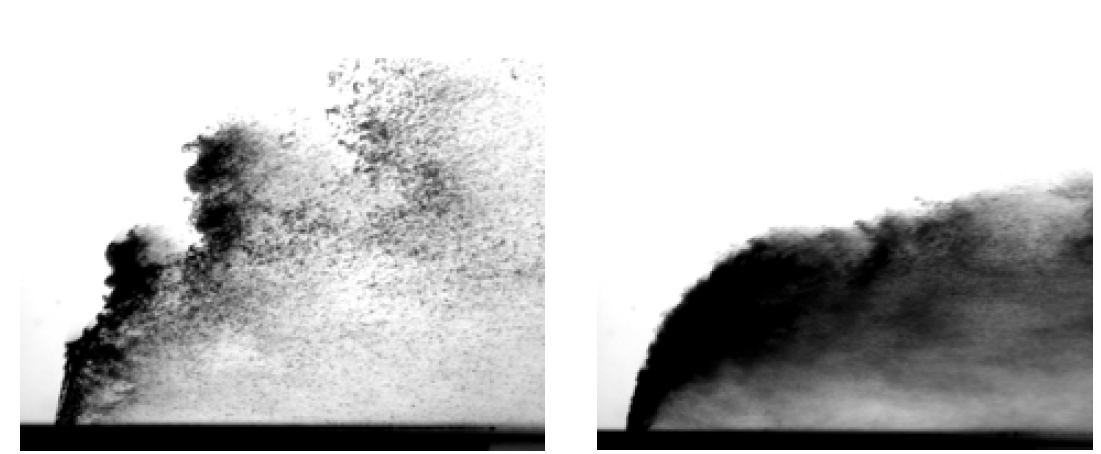
\includegraphics[scale=0.65]{./part0_intro/JICF_breakup-mechanisms_freitag}
	\caption[Experimental images of kerosene JICF breakup]{Experimental images of kerosene JICF breakup. \textsl{Left}: column breakup. \textsl{Left}: surface breakup. Source: \citeColor[freitag_spray_2008]}
	\label{fig:JICF_breakup_mechanisms_freitag}
\end{figure}

As in any two-phase problem, the physical and breakup characteristics of a JICF can be categorized by means of dimensionless numbers. In liquids jet in crossflow, the main two governing factors are the \textbf{momentum flux ratio} $q$ and the \textbf{Weber number based on the gaseouos phase} $We_g$, defined in Eq. (\ref{eq:q_and_We_JICF_parameters}). The former parameter represents the relation between the momentum, or kinetic energies, of the liquid and gaseous phases, while the latter represents the relative contribution of the gaseous phase to capillary forces. 

\begin{equation}
\label{eq:q_and_We_JICF_parameters}
	q = \frac{\rho_l u_l^2}{\rho_g u_g^2} ~~~~~~ ;  ~~~~~~ We_g = \frac{\rho_g u_g^2 d_\mathrm{inj}}{\sigma}
\end{equation}

The influence of these factors in the breakup process of liquid jets in crossflow has been experimentally studied by \citeColor[wu_breakup_1997], resulting in a breakup map of Figure \ref{fig:jicf_breakup_regime_wu}. Column and surface breakup, which are the main primary atomization regimes, are separated by the dividing line that indicates the transitional $q$ value between both regimes to be inversely proportional to $We_g$. For column breakup, several atomization modes appear depending on $We_g$. Figure \ref{fig:jicf_breakup_sallam} shows experimental snapshots of these modes. As displayed, for low $We_g$ (capillary and bag regimes) the breakup is dominated by capillary forces and the jet stays coherent until several nozzle diameters downstream the injection point, once the jet has bent and its cross section has been deformed. Waves are clearly observed in the windward side of the jet (i.e. the face in contact with the incoming air), and the wavelength of liquid surfaces $\lambda$ can be defined as the distance between two nodes.  For higher $We_g$ (multimode and shear regimes), instabilities causing breakup are also observed developing along the windward side of the jet, but it is also noticeable the stripping of liquid ligaments and droplets at the sides of the jets due to aerodynamic shear. For shear breakup these stripped-off structures appear close to the injection point, hindering the optical access to the jet structure and atomization characteristics further downstream. This was also observed for the surface breakup mode in Figure \ref{fig:JICF_breakup_mechanisms_freitag} right. Another noticeable characteristic is that the wavelengths $\lambda$ decrease for larger values of $We_g$. \citeColor[sallam_breakup_2004] found that the order of magnitudes of the wavelenghts with respect to the injection diameter is $\lambda/d_\mathrm{inj} > 1$ for capillary breakup, $\lambda/d_\mathrm{inj} \approx 1$ for bag breakup, $0.1 < \lambda/d_\mathrm{inj} < 1$ for the multimode regime and $\lambda/d_\mathrm{inj} \approx 0.1$ for shear breakup. The main responsible mechanisms of generating these surface waves are either Kelvin-Helmholtz or Rayleigh-Taylor instabilities. The former ones are said to be the dominating mechanisms for the waves observed in Figure \ref{fig:jicf_breakup_sallam} \citepColor[sallam_breakup_2004]. It is believed that the prevalence of either one or another mode depends on the density ratio between fluid and gas, being the Rayleigh-Taylor the main dominant mechanisms for high density ratios \citepColor[ghods_detailed_2013]. Nevertheless, the appearance and dependence of each instability mode is not certainly known nowadays and remains an open question requiring further research.

\begin{figure}[h!]
	\centering
	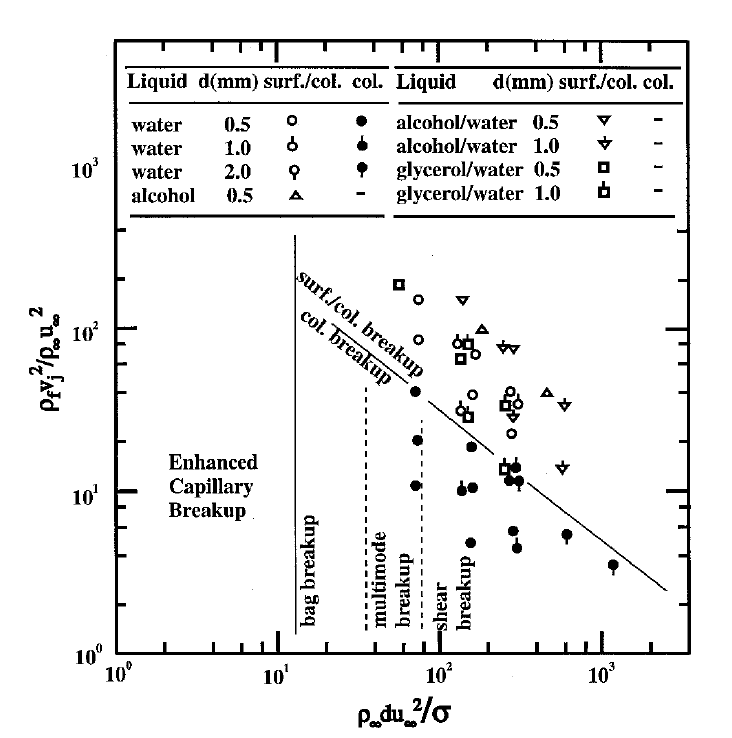
\includegraphics[scale=0.55]{./part0_intro/jicf_breakup_regime_wu}
	\caption{Breakup map for liquid jet in crossflow. Source: \citeColor[wu_breakup_1997]}
	\label{fig:jicf_breakup_regime_wu}
\end{figure}

\begin{figure}[h!]
	\centering
	\includeinkscape[inkscapelatex=true,scale=0.7]{./part0_intro/jicf_breakup_sallam}
	\caption[Primary breakup processes in liquid jet in crossflow]{Primary breakup processes in liquid jet in crossflow. Air flows from right to left. (a) No breakup, $We_g = 0$. (b) Capillary breakup, $We_g = 3$. (c) Bag breakup, $We_g = 8$. (d) Multimode breakup, $We_g = 30$. (e) Shear breakup, $We_g = 220$. Source: \citeColor[sallam_breakup_2004]}
	\label{fig:jicf_breakup_sallam}
\end{figure}

Another very important characteristic of the liquid jet in crossflow is its penetration, since in real configurations it will determine the region where evaporation and mixing takes place and, later, the flame structure. The near-field jet penetration can be quantified by means of the \textbf{vertical trajectory} of the jet, which is identified as the mean contour of its windward side. This trajectory can be experimentally obtained either from instantaneous snapshots of the jet (Figure \ref{fig:inst_and_mean_jets_ragucci} left) or from average images (Figure \ref{fig:inst_and_mean_jets_ragucci} right), each experimentalist using its own methods. From experimental studies, the trajectory is generally given by correlations relating the vertical trajectory $z$ with the axial coordinate $x$. Some experimental correlations are shown in Table \ref{tab:correlations_experimental_JICF}, where $We_{ae} = \rho_g u_l^2 d_\mathrm{inj}/\sigma$. Figure \ref{fig:inst_and_mean_jets_ragucci} right shows the jet correlation from \citeColor[ragucci_trajectory_2007] overlapped with the average jet view.


\begin{figure}[h!]
	\centering
	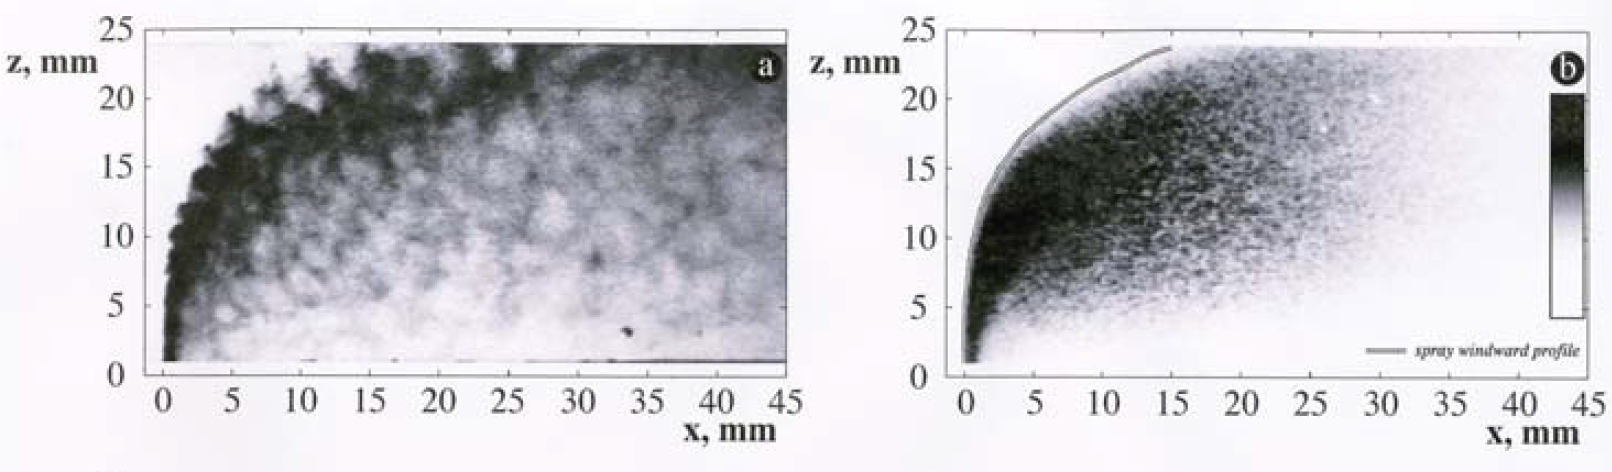
\includegraphics[scale=0.6]{./part0_intro/ragucci_jet_penetration}
	\caption{Instantaneous and averages images of a liquid jet in crossflow. Source: \citeColor[ragucci_breakup_2007]}
	\label{fig:inst_and_mean_jets_ragucci}
\end{figure}


\begin{table}[!h]
\centering
\caption{Correlations for the jet trajectory of the JICF}
\begin{tabular}{c|c|c|c}
\thickhline
$z / d_\mathrm{inj}$ & Liquid  & Range of validity & Reference  \\
\thickhline
\multirow{2}{*}{$1.37 \sqrt{q \left( \frac{x}{d_\mathrm{inj}} \right)}$} & \multirow{2}{*}{ Water } & $3.4 < q < 185$ & \multirow{2}{*}{\citeColor[wu_breakup_1997]} \\
& & $57 < We_{ae} < 1200$ & \\
\hline
\multirow{3}{*}{$1.57 \mathrm{q}^{0.36} \ln \left( 1 + 3.81 \frac{x}{d_\mathrm{inj}} \right)$} & \multirow{3}{*}{ Kerosene } & $1 < q < 12$  & \multirow{3}{*}{\citeColor[becker_breakup_2002]} \\
& & $90 < We_{ae} < 2120$ &  \\
& & $2 < x/d_\mathrm{inj}< 22$ & \\
\hline
\multirow{2}{*}{ $2.27 q^{0.44} We_{ae}^{-0.012} \left( \frac{x}{d_\mathrm{inj}} \right)^{0.367}$ }  & \multirow{2}{*}{Kerosene} & $5 < q < 280$  & \multirow{2}{*}{\citeColor[ragucci_trajectory_2007]} \\
& & $7 < We_{ae} < 340$ & \\
\hline
\multirow{3}{*}{ $1.6 q^{0.4} \ln \left( 1 + 3.81 \left( \frac{x}{d_\mathrm{inj}} \right) \right)$} & \multirow{3}{*}{Kerosene} & $3 < q < 24$ & \multirow{3}{*}{\citeColor[freitag_spray_2008]} \\
& & $39 < We_{ae} < 3281$ & \\
& & $1.4 < x/d_\mathrm{inj}< 50$ & \\
\thickhline
\end{tabular}
\label{tab:correlations_experimental_JICF}
\end{table}


%\begin{table}[!h]
%\centering
%\caption{Correlations for the jet trajectory of the JICF}
%\begin{tabular}{c|c|c|c}
%\hline
%$z / d_\mathrm{inj}$ & Liquid  & Range of validity & Reference  \\
%\hline
%\hline
%$1.37 \sqrt{q \left( \frac{x}{d_\mathrm{inj}} \right)}$ & Water & $3.4 < q < 185$ &\citeColor[wu_breakup_1997] \\
%\hline
%$2.27 q^{0.44} We_{ae}^{-0.012} \left( \frac{x}{d_\mathrm{inj}} \right)^{0.367}$   & Kerosene & $5 < q < 280$  & \citeColor[ragucci_breakup_2007] \\
%\hline
%\multirow{2}{*}{ $1.6 q^{0.4} \ln \left( 1 + 3.81 \left( \frac{x}{d_\mathrm{inj}} \right) \right)$} & \multirow{2}{*}{Kerosene} & $3 < q < 24$ & \multirow{2}{*}{\citeColor[freitag_spray_2008]} \\
%& & $1.4 < x/d_\mathrm{inj}< 50$ & \\
%\hline
%\end{tabular}
%\label{tab:correlations_experimental_JICF}
%\end{table}


In general, all the correlations from Table \ref{tab:correlations_experimental_JICF} show a dependence of the jet trajectory with the injection diameter $d_\mathrm{inj}$ and the momentum flux ratio $q$. These are the two main parameters governing the jet penetration. The larger the injection diameter, the further the jet will penetrate. This is attributed to a more coherent jet: if $d_\mathrm{inj}$ increases, more liquid mass flow is injected, so the jet carries more momentum and is able to withstand more stiffly the
interaction with the airstream. Furthermore, atomization of a thicker jet will produce larger droplets that
will travel further due to their ballistic properties. For the momentum flux ratio, increasing its value also increases the jet penetration. This is clearly seen in Table \ref{tab:correlations_experimental_JICF}, as the exponent factor of $q$ is positive in all correlations. Figure \ref{fig:parametric_JICF_q_ratio} shows the $q$ effect in the jet penetration. Regarding the influence of the air velocity (or equivalently, $We_g$), it does not have a direct effect in the jet penetration close to the injection nozzle, as the correlations from Table \ref{tab:correlations_experimental_JICF} do not show any dependence with $We_g$. This is observed in Figure \ref{fig:parametric_JICF_air_velocity}, which shows instantaneous snapshots of a liquid JICF for several values of $u_g$. The main effect of increasing the gas velocity is the transition from column to surface breakup mechanisms, as given by the breakup map of Figure \ref{fig:jicf_breakup_regime_wu}. Nevertheless, it is seen that by increasing $u_g$, the far-field penetration is reduced due to a finer atomization: for low values of $u_g$, column breakup generates bigger droplets whose ballistic properties allow them to penetrate further in the vertical direction, while higher values of the gas velocity generate smaller droplets both from surface and column breakup mechanisms that will relax faster towards the air velocity and direction. \citeColor[becker_breakup_2002] tested a kerosene JICF with several gas velocities and measured the granulometry of the developed spray at a plane located 80 mm downstream the injection nozzle, obtaining the following relation between the Sauter Mean Diameter (SMD) and the kinetic energy of the gas which confirms how the mean droplet size decreases with increasing gas velocity:

\begin{equation}
SMD = 429 \left( \rho_g u_g^2 \right)^{-0.24}
\end{equation}



\begin{figure}[h!]
	\centering
	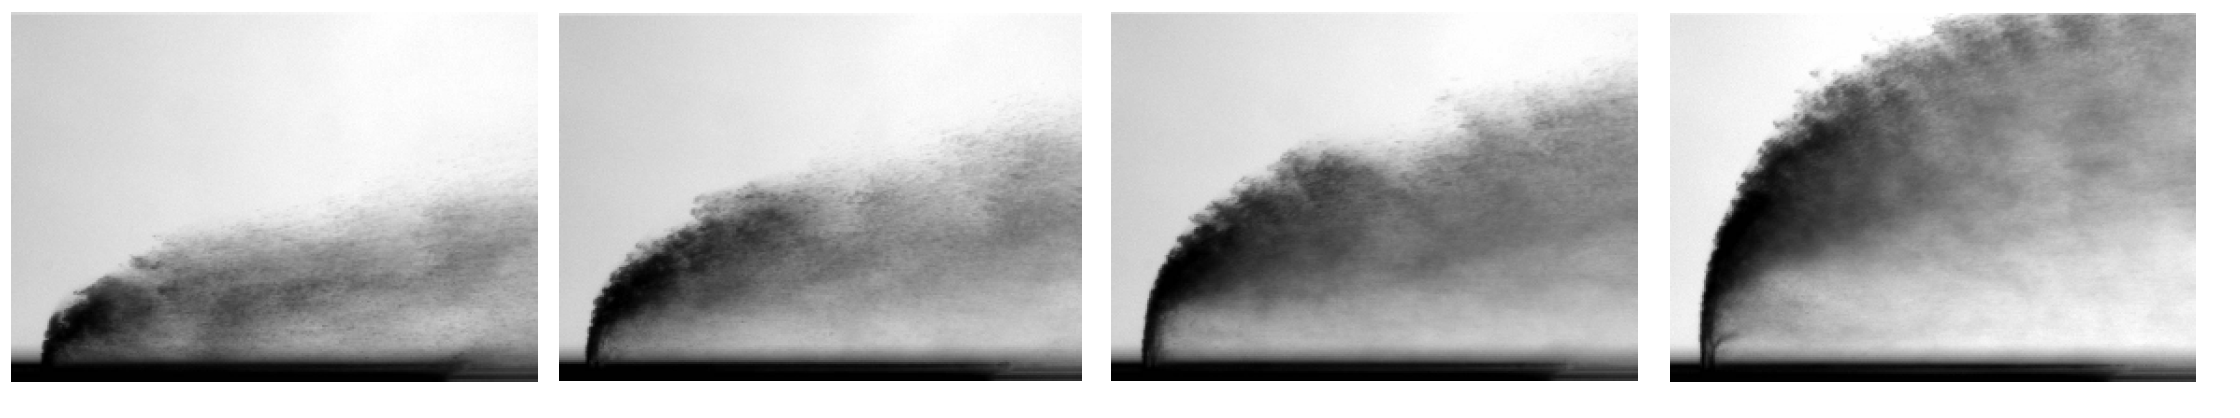
\includegraphics[scale=0.45]{./part0_intro/parametric_JICF_q_ratio}
	\caption{Effect of $q$ ratio. From left to right: $q = 3, 6, 12, 24$. Fixed values: $d_{inj} = 0.5 ~mm$, $u_g = 75 ~m/s$, $p_\infty = 4 ~\mathrm{bar}$. Source: \citeColor[freitag_spray_2008].}
	\label{fig:parametric_JICF_q_ratio}
\end{figure}

\begin{figure}[h!]
	\centering
	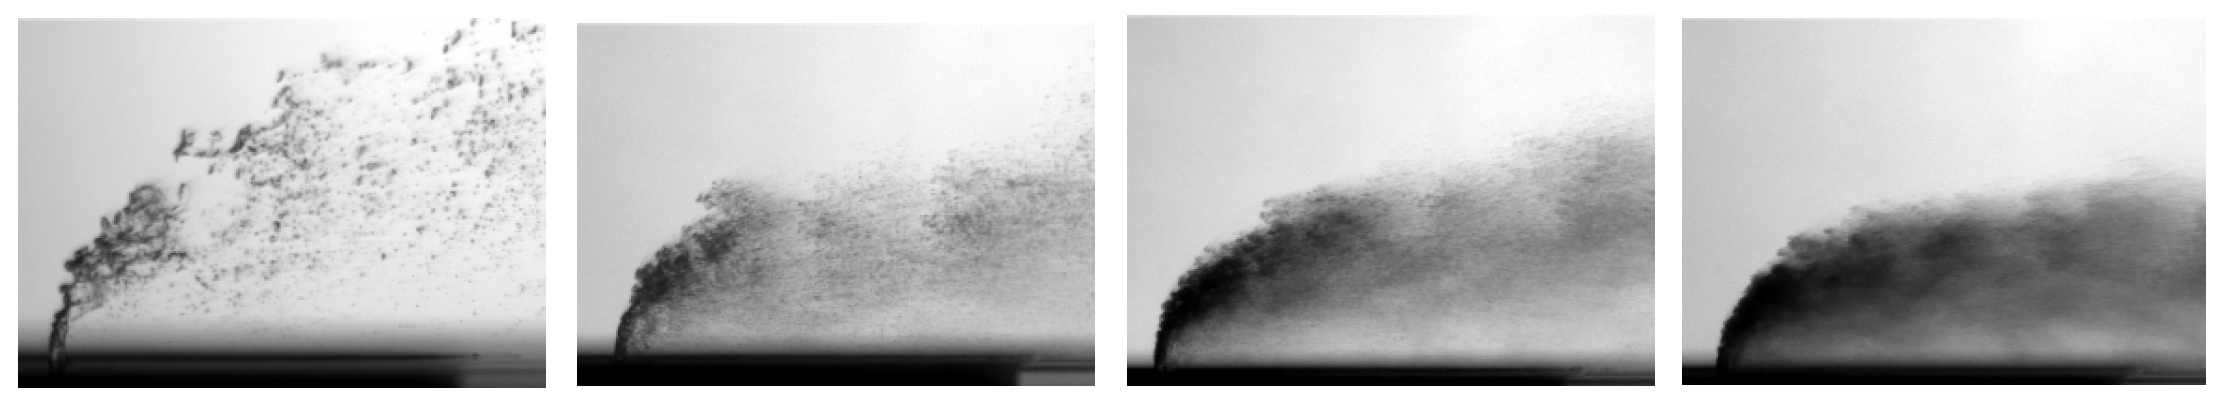
\includegraphics[scale=0.45]{./part0_intro/parametric_JICF_air_velocity}
	\caption{Effect of air velocity. From left to right: $u_g = 25, 50, 75, 100 ~m/s$. Fixed values: $d_{inj} = 0.5 ~mm$, $q = 6$, $p_\infty = 4 ~\mathrm{bar}$. Source: \citeColor[freitag_spray_2008].}
	\label{fig:parametric_JICF_air_velocity}
\end{figure}

%Regarding internal nozzle effects Internal nozzle effects: effect of L/D ratio, some words on cavitation and hydraulic flip (ref. Chemloul).

\section{Numerical simulations of fuel injection and combustion }

The previous section has illustrated the heterogeneity of phenomena which are found in injection systems relevant to gas turbines, with a special focus on MSFI technology aiming at reducing NO$_\mathrm{x}$ formation. The study of these phenomena with experimental facilities is often restricted to academic cases without complex geometries due to difficult optic visualization. Furthermore, experiments do not have access to all the magnitudes of interest relevant to the problem, and some cases dealing with combustion they can involve safety issues.

An alternative to study and design injection and combustion systems is the use of numerical simulations with Computational Fluid Dynamics (CFD). This tool has gained popularity in the last decades due to the increase in computational performances and the appearance of High Performance Computing (HPC), which allows to perform simulations of complex problems in parallel machines. CFD simulations can provide insightful information in the physical mechanisms and variables of interest, they do not have limitations regarding optical access and are hazard-free. Therefore, numerical simulations have become a powerful tool for the design of combustion systems and the understanding of the underlying fundamental physical phenomena.

In order to resolve a given physical problem, the proper modeling strategy and numerical methods to perform CFD simulations must be chosen. Depending on the required accuracy and the computational resources available, three main approaches exist to resolve numerically the Navier-Stokes equations. From lower to higher accuracy (and equivalently, from lower to higher computational cost), these approaches are:

\begin{enumerate}

	\item \textbf{Reynolds Averaged Navier Stokes} (RANS). The governing equations are averaged and the mean flow field is solved. Extra terms appear in the equations which need mathematical closure. All the turbulence spectrum, from Taylor to Kolmogorov characteristic length scales, is modeled. RANS can provide mean values and are good to characterize pressure drop in certain configurations, but are not suited for solving transient problems.
	
	\item \textbf{Large-Eddy Simulations} (LES). A low-pass filter is applied to the Navier-Stokes equations, so that the characteristic length scales below the filter size are modeled and the larger ones are resolved. For the smallest scales, turbulence models are required which accounts for the viscous dissipation. One of the most well-known filters is the Smagorinsky model \citemColor[smagorinsky_general_1963,germano_dynamic_1991].
	
	\item \textbf{Direct Numerical Simulations} (DNS). In such simulations, all the turbulence characteristic scales are solved and no models are applied. Hence, DNS is an accurate tool for properly resolving turbulence. Nevertheless, its high computational cost reduces the application of DNS to reduced geometries and canonical test cases, and nowadays its application to full industrial configurations is out of reach.

\end{enumerate}

These three methodologies are widely used for aerodynamic and hydrodynamic problems involving one fluid phase. Two-phase flow problems also make use of these equations, but they require additional equations and modeling tools to consider the interaction between phases. For cases involving liquid and gas, which are of interest in automotive and aeronautical engines, this interaction is dominated by surface tension $\sigma$. In terms of numerical modeling, surface tension creates a discontinuity in pressure and viscosity (as demonstrated later in $\S$\ref{sec:ch2_governing_equations}) that needs to be dealt with mathematical tools, for instance by adding extra forcing terms in the governing equation for momentum. Furthermore, different methods and modeling methodologies will be used depending on the problem to solve, since the multi-scale, complexity and richness of the physical phenomena in two-phase flows (illustrated in $\S$\ref{sec:ch1_fuel_injection_technology}) does not allow to use a single numerical formalism to solve simultaneously all processes involved.

One large family of numerical methods is the one devoted to resolve accurately atomization. The underlying interest is to capture the dynamics of primary and secondary atomization, its governing physical mechanisms and the interaction with the gaseous phase. For this purpose, the main approach is to perform CFD simulations where the Navier-Stokes equations are resolved for each phase with RANS or LES. Then, additional equations are added in order to determine either the evolution of the interface (e.g. level-set methods) or of the liquid volume fraction (e.g. volume of fluid methods). These simulations are usually denoted as \textbf{resolved} or \textbf{eulerian}. Figure \ref{fig:DNS_simulations_jets} shows two instantaneous jets solved with a resolved atomization approach, where the interface dynamics have been solved with level-set methods. A diesel jet coloured by axial velocity and a liquid jet in crossflow are shown. In both cases, ligaments and droplets generated by the atomization process can be clearly appreciated. In this document, Chapter \ref{ch2:numerical_methods_resolved_atomization} presents numerical methods used nowadays for resolving injection and atomization.

\begin{figure}[h!]
	\centering
   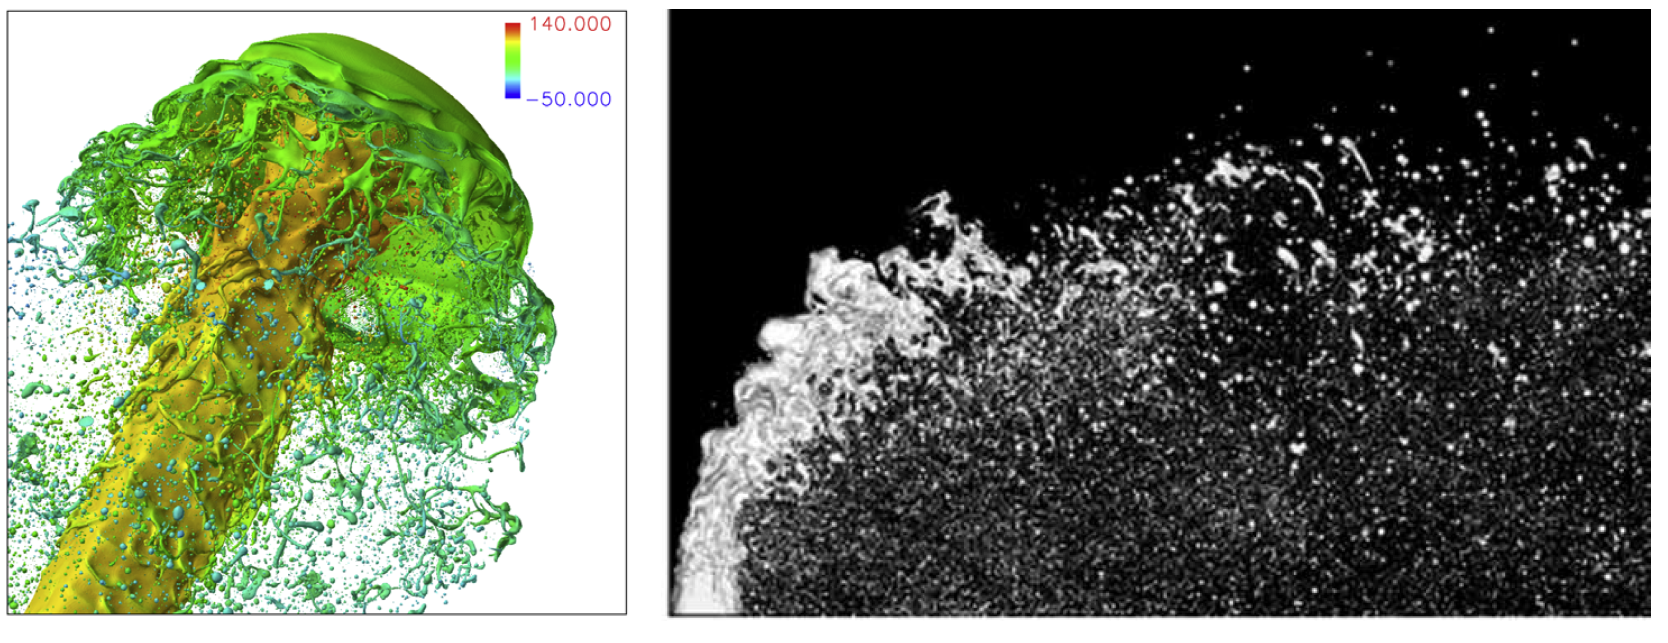
\includegraphics[scale=0.4]{./part0_intro/jets_DNS_simulations}
	\caption[Direct numerical simulations of primary atomization in liquid jets.]{Direct numerical simulations of primary atomization in liquid jets. \textsl{Left}: diesel jet, from \citepColor[shinjo_simulation_2010]. \textsl{Right}: liquid jet in crossflow, from \citeColor[herrmann_detailed_2009].}
	\label{fig:DNS_simulations_jets}
\end{figure}

Methodologies for resolving atomization are envisaged to capture the multi-scale nature of atomization, devoting huge computational resources to solve from the biggest to the smallest scales and the interaction between phases. Nevertheless, the size of the smallest structures and droplets captured are often limited by the grid resolution, and due to their high cost cannot be easily coupled with additional physical equations to solve for the evaporation and combustion processes. To tackle these problems, different strategies are used, often circumventing atomization by injecting a spray represented by liquid spherical particles. These particles compose a \textbf{dispersed-phase system} where the gaseous phase is resolved by the Navier-Stokes equations and the particles representing the liquid phase evolve according to the dynamics of point-particle systems in \textbf{lagrangian simulations}. The coupling between both phases is done through exchange terms of mass, momentum and energy, and hence evaporation and combustion can be easily modelled in these simulations. Figure \ref{fig:lagrangian_simulations_jets} shows also two jets, diesel and jet in crossflow, simulated with lagrangian approaches. Contrarily to the resolved jets of Figure \ref{fig:DNS_simulations_jets}, here all the liquid phase is represented by means of spherical particles and the dynamics of atomization are not appreciated. In contrast, these simulations are computationally much cheaper than the former ones and can be applied to reactive computations in complex geometries as shown in Figure \ref{fig:reactive_LES_combustor_Moin}, where a full combustor is studied. In lagrangian simulations, the injection process is fundamental and needs to be properly modeled by injecting the right droplets sizes and velocities distributions. Chapter \ref{ch3:disperse_phase_methods} shows the state of the art on several numerical tools to approach dispersed two-phase phase systems, with special emphasis on their application to approach liquid jet in crossflow injection.

\begin{figure}[h!]
	\centering
   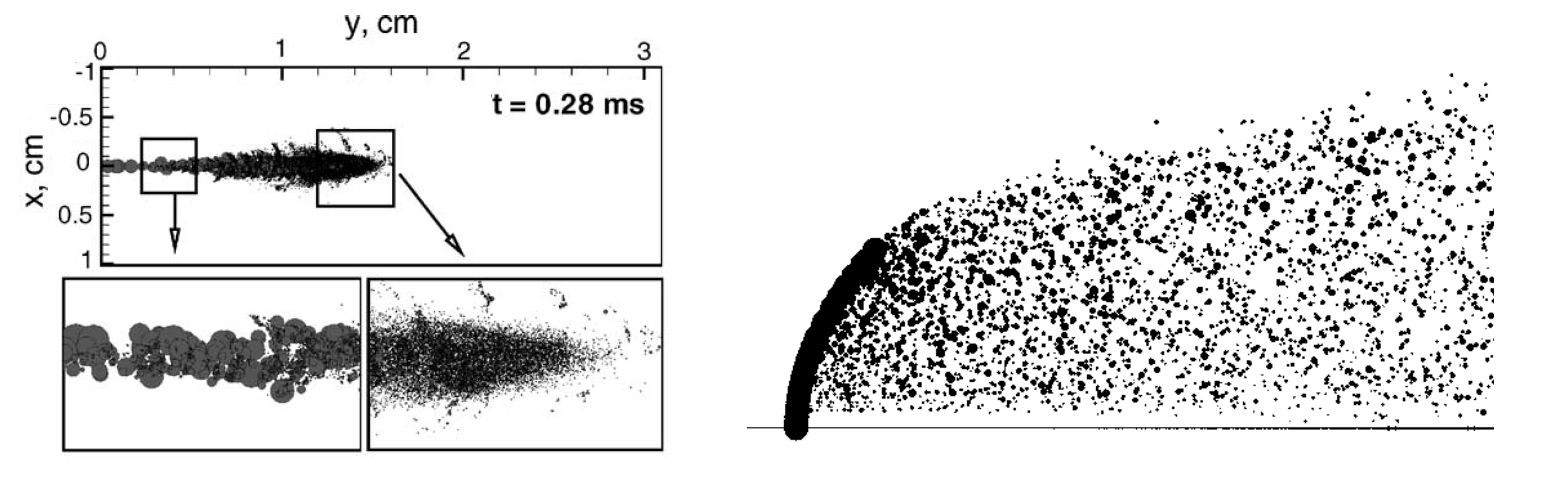
\includegraphics[scale=0.5]{./part0_intro/jets_lagrangian_simulations}
	\caption[Lagrangian simulations of liquid jets.]{Lagrangian simulations of liquid jets. \textsl{Left}: diesel jet, from  \citeColor[apte_les_2003]. \textsl{Right}: liquid jet in crossflow, from \citeColor[behzad_kiva-based_2010].}
	\label{fig:lagrangian_simulations_jets}
\end{figure}

\begin{figure}[h!]
	\centering
   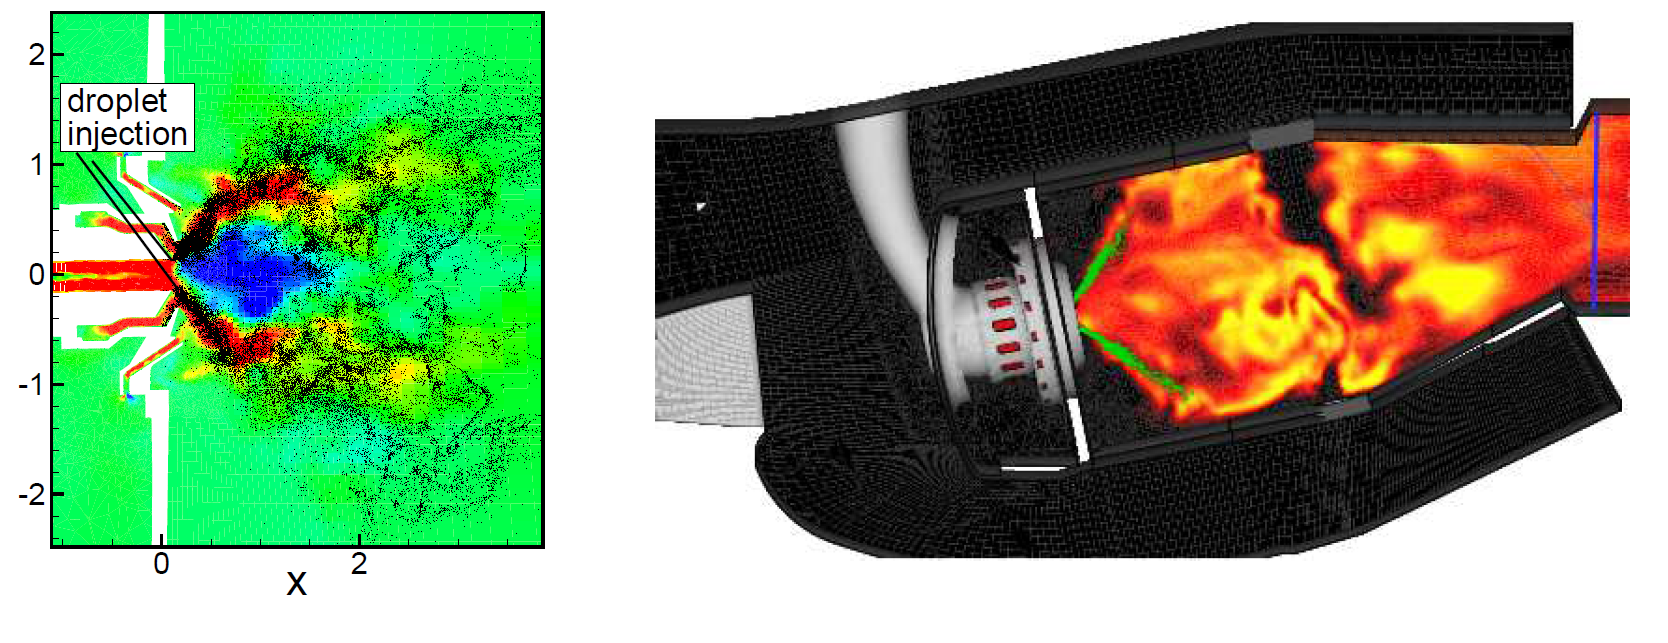
\includegraphics[scale=0.45]{./part0_intro/reactive_LES_combustor_Moin}
	\caption[Large Eddy Simulation of a Pratt \& Whitney combustor.]{Large Eddy Simulation of a Pratt \& Whitney combustor. \textsl{Left}: fuel spray injection, where liquid phase is represented by lagrangian droplets. \textsl{Right}: combustion simulation. Source: \citeColor[moin_large-eddy_2006].}
	\label{fig:reactive_LES_combustor_Moin}
\end{figure}

Recently, new methodologies have emerged to represent more accurately the spray by coupling dispersed phase with lagrangian simulations. \citeColor[michaelides_multiphase_2017] make a distinction of these coupling methodologies in two main categories: Direct Coupling Approach (DCA) and Statistical Coupling Approach (SCA), shown in Figure \ref{fig:coupled_EE_EL_approaches_Michaelides}. In DCA, primary atomization is simulated with eulerian approaches, and resolved eulerian droplets are transformed into spherical droplets which are later transported with the lagrangian equations. Conversion criteria based on droplets size and sphericity are used. This approach has been studied by several authors who have demonstrated its capabilities to simulate non-reactive problems \citemColor[herrmann_parallel_2010,zuzio_improved_2018,janodet_numerical_2022], but has not yet been applied to combustion cases. In SCA, an eulerian simulation resolves the jet up to a plane after atomization has taken place where droplets are sampled (SC layer in Figure \ref{fig:coupled_EE_EL_approaches_Michaelides}). Then, the information on the sampled spray is used to inject lagrangian droplets, which are then transported further downstream.

\begin{figure}[h!]
	\centering
   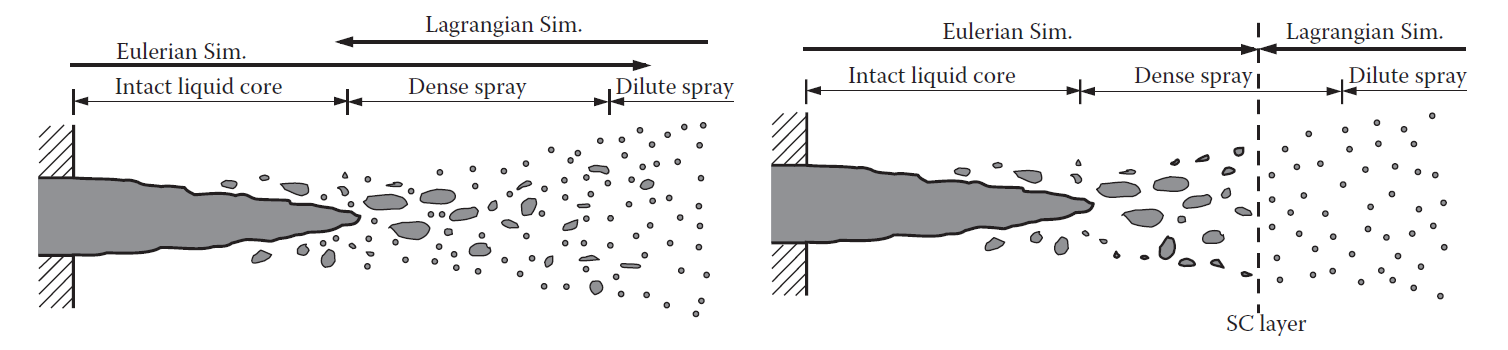
\includegraphics[scale=0.5]{./part0_intro/coupled_EE_EL_approaches_Michaelides}
	\caption[Schematic of coupled Eulerian–Lagrangian approaches for liquid atomization.]{Schematic of coupled Eulerian–Lagrangian approaches for liquid atomization. \textsl{Left}: direct coupling approach, DCA. \textsl{Right}: statistical coupling approach, SCA. Source: \citeColor[michaelides_multiphase_2017].}
	\label{fig:coupled_EE_EL_approaches_Michaelides}
	% Michaelides, p. 1140
\end{figure}


\section{Objective and thesis outline}
\label{sec:ch1_objective_thesis_outline}
    %\addcontentsline{toc}{section}{\protect\numberline{}Manuscript organisation}

The interest in performing lagrangian simulations to study combustion within gas turbines has seen a huge increase in the recent decades due to the potential of this methodology for modeling multi-physics problems with reduced computational costs. To accurately perform such simulations, lagrangian particles need to be properly injected by prescribing droplets sizes and velocities in the right spatial location. Often, distributions measured experimentally are in prescribed such simulations to recover the dispersed spray obtained further downstream \citepColor[jaegle_large_2009]. This requires the availability of experimental test benches representative of the geometry and operating conditions simulated, which is not always possible. Other approaches inject directly droplets with the diameter of the injector and the velocity at injection, coupling with secondary breakup models to form a developed spray \citepColor[reitz_modeling_1987], with the disadvantage that primary atomization is not considered. Intermediate approaches combine the injection of large droplets with semi-empirical models to take into account more realistic physics \citepColor[eckel_semi-empirical_2016], allowing to obtain a more realistic spray but being applicable to a few range of operating conditions. Furthermore, most of the models applicable to reactive simulations fail into taking into account the interaction between the aerodynamic and the liquid, and available models considering this interaction \citemColor[arienti_aerodynamic_2006,fontes_improved_2019] combine resolved atomization methods with dispersed phase ones in one simulation, hindering the application to combustion problems. A thorough review of lagrangian injection models in MSFI systems in done in Chapter \ref{ch3:disperse_phase_methods}.

    
The goal of this thesis is to develop a new methodology to build lagrangian injectors for performing dispersed phase simulations which prescribe a realistic spray in MSFI systems, with a final application to reactive simulations. For this purpose, in first place resolved simulations of an academic liquid JICF configuration tested experimentally \citepColor[becker_breakup_2002] are performed with an Accurate Conservative Level Set formalism \citepColor[desjardins_accurate_2008] to construct a database of atomization representative of MSFI. The methodology makes use of this database in order to learn the spray state and construct the injectors for initialising dispersed phase simulations. The developmed methodology is similar to the SCA approach from Figure \ref{fig:coupled_EE_EL_approaches_Michaelides}. Apart from the atomization data, the aerodynamic interaction is also taken into account by means of the Actuator Line Method (ALM) \citepColor[sorensen_numerical_2002]. Then, the methodology is validated by performing dispersed phase simulations in the same configuration. In a second step, the methodology is applied to an academic burner called BIMER which is more representative of industrial MSFI configurations \citepColor[renaud_high-speed_2015]. \\

%This thesis has been performed with Safran Group under the ITN programme ANNULIGhT, funded by the H2020 Marie Curie actions. The manuscript is divided in three main sections as follows:

The manuscript is divided in three main sections as follows:

\begin{itemize}

	\item \textbf{Part I} shows the state of the art in numerical methods to simulate two-phase flows. Different strategies are used depending on the atomization regimes as shown in Figure \ref{fig:atomization_regimes_herrmann}. Chapter \ref{ch2:numerical_methods_resolved_atomization} reviews methodologies aiming at resolving atomization, applicable to dense regimes and useful when the atomization dynamics need to be known, but out of scope for reactive simulations including combustion. Chapter \ref{ch3:disperse_phase_methods} discusses methodologies to simulate dispersed-phase problems, with a particular emphasis on the state of the art in lagrangian methodologies to simulate injection in MSFI.
	
	\item \textbf{Part II} describes the design and application of the methodology developed in this thesis. This methodology is thoroughly described in Chapter 4. Then, application of this methodology to build lagrangian injectors in an academic non-reactive kerosene jet in crossflow test case is done in Chapter 5. The obtained injectors are then applied in the same configuration to initialise dispersed phase simulations in Chapter 6.
	
	\item \textbf{Part III} focuses on the application of the injection models in an academic MSFI tested at EM2C named BIMER. An introduction to the test bench and simulations of the aerodynamic field are presented in Chapter 7. Then, Chapter 8 describes resolved simulations of the atomization process in BIMER performed for one multipoint injector, from which lagrangian injectors are learnt. Finally, Chapter 9 shows the application of the built injectors to initialise lagrangian simulations in the BIMER burner.

%	\item \textbf{Part I} shows the state of the art in numerical methods to simulate two-phase flows. Different strategies are used depending on the atomization regimes as shown in Figure \ref{fig:atomization_regimes_herrmann}. Chapter \ref{ch2:numerical_methods_resolved_atomization} reviews methodologies aiming at resolving atomization, applicable to dense regimes and useful when the atomization dynamics need to be known, but out of scope for reactive simulations including combustion. Chapter \ref{ch3:disperse_phase_methods} discusses methodologies to simulate dispersed-phase problems, with a particular emphasis on the state of the art in lagrangian methodologies to simulate injection in MSFI.
%	
%	\item \textbf{Part II} describes the design and application of the methodology developed in this thesis. This methodology is thoroughly described in Chapter \ref{ch4:sli_development}. Then, application of this methodology to build lagrangian injectors in an academic non-reactive kerosene jet in crossflow test case is done in Chapter \ref{ch5:jicf_resolved_simulations}. The obtained injectors are then applied in the same configuration to initialise dispersed phase simulations in Chapter \ref{ch4:sli_development}.
%	
%	\item \textbf{Part III} focuses on the application of the injection models in an academic MSFI tested at EM2C named BIMER. An introduction to the test bench and simulations of the aerodynamic field are presented in Chapter \ref{ch9:bimer_test_bench_and_aero}. Then, Chapter \ref{ch8:bimer_resolved_atomization} describes resolved simulations of the atomization process in BIMER performed for one multipoint injector, from which lagrangian injectors are learnt. Finally, Chapter \ref{ch9:BIMER_lagrangian} shows the application of the learnt injectors to initialise lagrangian injection in the take-off stage of BIMER.

\end{itemize}

